\chapter{Quantitative Correlation of Extreme Ultraviolet Magneto-Optic and Photoemission Spectroscopies}
\label{PRLchap}
In this chapter, we investigate the ultrafast magnetic phase transition in Ni using time-resolved transverse- magneto- optical Kerr effect (TR TMOKE) spectroscopy based on high harmonic generation. Using the critical behavior and the timescales of demagnetization and recovery processes observed from TR ARPES, and by taking the depth- dependent signal contributions in TR TMOKE into account, we show that critical phenomena are also key for the correct interpretation and a full understanding of ultrafast optical or x-ray magnetic spectroscopies. With this knowledge, we can now fully explain the TR- TMOKE response of Ni over the full range of laser fluences, using only three universal timescales to describe the demagnetization and recovery dynamics in distinct physical regions. Although the spin system absorbs all the energy required to proceed through a magnetic phase transition within 20 fs, the spectroscopic signatures of demagnetization take ∼176 fs to develop. Moreover, these timescales are fluence independent. In contrast, the speed of remagnetization dynamics depends on whether the applied laser fluence is below or above the critical fluence. Our data show that the demagnetization amplitudes scale linearly with pump fluence. Finally, we observe a competition between the fast and slow recovery channels with distinct timescales, suggesting a potential coexistence of ferromagnetic and paramagnetic phases during the phase transition.


A schematic of the physics studied in the experiment is shown in Fig. \ref{fig:PRLfig1}. The sample used in our experiments was a 400 nm Ni(111) single-crystal film. We intentionally chose a thick film sample to minimize nonlocal effects due to interfaces or poor substrate thermal conduction [29,30] and also verified that the observed dynamics were not dependent on the orientation of the sample (see the Supplemental Material [31]). In both the TR-TMOKE and TR-ARPES experiments, the sample was excited by 45 fs pulses from a Ti:sapphire laser amplifier system at a wavelength of 800 nm. In the TR-TMOKE measurements, the subsequent change of the sample magnetization was probed by extreme ultraviolet (EUV) pulses produced by high harmonic generation (HHG). The sample magnetization can be quantitatively determined by recording the asymmetry of the reflected HHG spectrum at the 3p edge of Ni [6,7,11]. In the TR-ARPES measurements, the magnetization dynamics was probed by monitoring the magnitude of the exchange splitting at different time delays [2,8,27].

In order to determine if Tr-TMOKE and Tr-ARPES give spectroscopic signatures that are consistent with the same microscopic physics and interactions, we measured the de- and remagnetization dynamics in Ni excited by a wide range of fluences, with the highest fluence sufficient to fully suppress the TR-TMOKE asymmetry (i.e., demagnetize the sample). The pump penetration depth in Ni is $\delta$L $\approx$ 13 nm [41], which is comparable to the probing depth of the EUV light used in the TR-TMOKE experiments (10 nm). In contrast, the probing depth of photoelectrons is close to a monolayer for the photon energy (16 eV) used in the TR- ARPES experiments [42], which suggests that the TR- ARPES signal can probe the elementary magnetization dynamics in an individual surface layer of the sample. In Fig. \ref{fig:PRLfig1}(b), we conceptually summarize the electron, spin, and magnetization dynamics after laser excitation, with the critical behavior taken into consideration [27].

\begin{figure}
	\label{fig: PRLfig1}
\begin{center}
	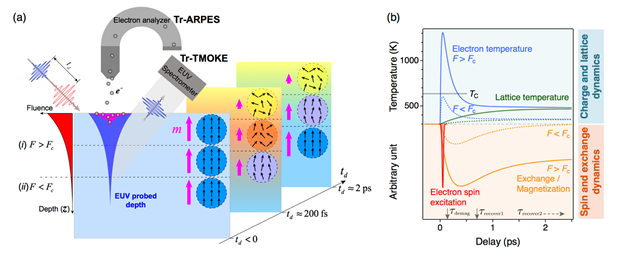
\includegraphics[width=150mm]{figs/PRLFig1}
\end{center}
\caption{(a) Schematic of EUV ARPES and TMOKE measurements on Ni(111). The fluence profile of the laser excitation below the sample surface separates the magnetization response into two different regions (i) and (ii), depending on whether the in-situ fluence is above the critical fluence $F_c$. Using TR ARPES, the probed depth is on the order of a monolayer, while TR-TMOKE probes the entire laser-heated depth of $\approx$10 nm. (b) Schematic of the excitation present in the laser-induced phase transition in Ni when critical phenomena are taken into consideration [27]. When the laser fluence exceeds the critical fluence $F_c$, the electron temperature exceeds $T_c$ and the sample rapidly undergoes a magnetic phase transition, as evidenced by multiple critical phenomena.}
\end{figure}

\begin{figure}
	\label{fig: PRLfig2}
	\begin{center}
		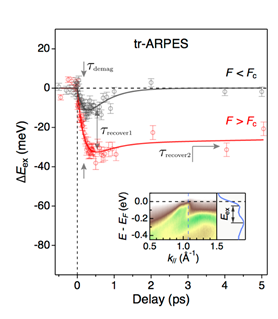
\includegraphics[width=75mm]{figs/PRLFig2}
	\end{center}
	\caption{Change in the exchange splitting ($\Delta E_{ex}$) in Ni measured using TR ARPES, for the absorbed laser fluence below (0.21 mJ = c$m^2$, grey) and above (1.7 mJ = c$m^2$, red) the critical fluence $F_c$. The solid lines are the fits to Eq. \ref{eqn:5.1}. Inset: Static ARPES spectrum plot along the $\Gamma$ − K direction recorded using He $I_{\alpha}$ photons.}
\end{figure}

In Fig. \ref{fig: PRLfig2}, we plot the change of the exchange splitting ($\Delta E_{ex}$) at the transverse momentum $k_{\/\/}$ $\approx$ 1.05 $\AA^{−1}$ along the $\Gamma$ - K direction of Ni (inset of Fig. \ref{fig: PRLfig2}) observed in the TR-ARPES measurements [27]. Due to $<$1 nm probing depth, TR ARPES probes the elementary magnetization dynamics in a monolayer of the material, which can be well described by an exponential decay and biexponential recovery function as shown in Fig. \ref{fig: PRLfig2}:
	
\begin{equation*}
Y(t_{d}) = 
\begin{cases}
1  \; (t_d<0)\\
1 + a_1(z) e^{-t_d\/\tau_{demag}}-a_2(z) e^{-t_d\/\tau_{recover1}}-a_3(z) e^{-t_d\/\tau_{recover2}} \; (t_d\geqslant)
\end{cases}
\label{eqn:5.1}
\end{equation*} 


Here we obtain three time constants that correspond to the following physical processes: the collapse of the exchange splitting $\tau_{demag}$ =  176 $\pm$ 27 fs, a fast recovery time $\tau_{recover1}$ = 537 $\pm$ 173 fs, and a slow recovery time [31] for data supporting the extraction of the time constants. $\tau_{recover2}$ = 76 $\pm$ 15 ps [27]. See the Supplemental Material In Eq. \label{eqn:1}, $a_1$, $a_2$, and $a_3$ are the amplitudes of these amplitudes are independent since the magnetization will processes, with $a_1$ = $a_2$ + $a_3$. Note that only two of the recover fully at long times. Their values depend on the strength of the laser fluence and, hence, are depth dependent due to the profile of the optical pump below the sample surface [Fig. \ref{fig: PRLfig1}(a)]. From the ARPES results, we map the dynamics in monolayers of the material—we can now test whether this understanding can fully explain the TR- TMOKE results.

The magnetization dynamics in the same sample excited by fs laser irradiation were also measured using TR TMOKE. In the inset of Fig. \ref{fig: PRLfig3}, we present the bulk-averaged hA2i, and hA3i) as a function of pump fluences, by fitting averaged amplitudes of de- and remagnetization ($<A_1>$, $<A_2>$, $<A_3>$) as a function of pump fluences, by fitting the TR-TMOKE results presented in Fig. \ref{fig: PRLfig3} with the same exponential decay and bi-exponential recovery function. Here the amplitudes represent the change of the sample magnetization normalized to the magnetization of the ground state. Even from the raw data traces, the presence of three timescales is very apparent: a fast and universal demagnetization time followed by fast and slow recoveries depending on the fluence.  From these results, we find that the slow-recovery process ($<A_3>$) only turns on when the absorbed laser fluence ($F_{abs}$) is above the critical fluence ($F_c$ $\approx$ 0.59 mJ/c$m^2$), which highlights the importance of the critical behavior to the interpretation of the Tr-TMOKE results (Note that in [25] we quoted the incident fluence of 2.8 mJ/c$m^2$, which is consistent with an absorbed fluence of 0.59 mJ/c$m^2$ within error bars). Moreover, a linear response of the slow-recovery amplitude  can be clearly observed, as highlighted in the inset of Fig. \ref*{fig: PRLfig3}.

\begin{figure}
	\label{fig: PRLfig3}
	\begin{center}
		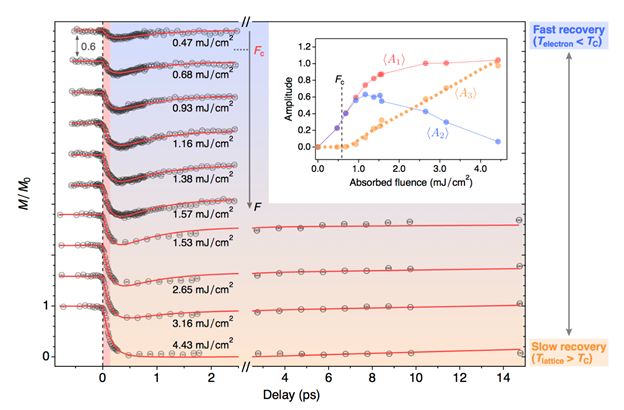
\includegraphics[width=150mm]{figs/PRLFig3}
	\end{center}
\caption{Magnetization dynamics in Ni measured using TRTMOKE over a full range of laser fluences. The highest fluence is sufficient to fully suppress the sample magnetization. The data are offset for clarity. Red curves: Fits to our microscopic model which considers the critical behavior, as well as the depth-average effects in the TR-TMOKE measurements. Inset: Fluence-dependent amplitudes of the demagnetization and recovery processes directly extracted from the TR-TMOKE results. In the TR-TMOKE results, the magnetization $<M>$ and the extracted amplitudes $<A_1>$, $<A_2>$, and $<A_3>$ are averaged over the entire probed depth (see text). The dashed yellow line highlights the linear relation of the amplitude $<A_3>$ to the absorbed fluence when the fluence is above the critical fluence.}
\end{figure}

Under the assumption of linear absorption, in both experiments the in-situ laser fluence F decays exponentially with the depth z i.e. F(z) = $F_0 e^{z/\delta_L}$, where $F_0$ is the fluence at the surface. To take into account the true absorption at different depths, the heat source q can be calculated by q(z)=F(z)/$\delta_L$. When  $F_0 > F_c$, the Tr-TMOKE signal arises from different regions, each exhibiting different recovery dynamics depending on whether the laser excitation is above or below the critical fluence (Fig. \ref{fig: PRLfig1}a). In Region (i) where the in-situ fluence is always lower than the critical fluence, and the sample re-magnetizes through the fast recovery channel. In contrast, in Region (ii), the in-situ fluence is above $F_c$, and re-magnetization occurs through both slow and fast recovery channels.  Here, we further assume that the change of magnetization is a linear function of the in-situ fluence, which is strongly supported by our experimental results (inset of Fig. \ref{fig: PRLfig5.3}) and previous work [28]. Given this linear relation, we have 

\begin{equation}
a_1(z) = \textbf{min}[b_1 \: F(z),1]
\label{eqn:5.2}
\end{equation}
and
\begin{equation*}
a_3(z) = 
\begin{cases}
0 \; \left[F(z) < F_c\right]\\
\text{min} \left[ b_3 \left[ F(z)-F_c \right] \right]; \left[F(z) \geq F_c\right]
\end{cases}
\label{eqn:5.3}
\end{equation*}

where $b_1$ and $b_3$ are the proportionality constants. The Tr-TMOKE signals can be modeled as the bulk-averaged magnetization $<M>$, given by the integral of the unit magnetization m($t_d$, z) over the probed depth z:

\begin{equation}
<M>(t_d)=\frac{\int^{\infty}_0 m(t_d,z) W(z) dz}{\int^{\inf}_0 W(z) dz}
\label{eqn:4}
\end{equation}

Here, W(z) is the depth sensitivity function of TMOKE [44], which is explicitly calculated for Ni (see the Supplemental Material [31] for details).

Using the model described above, we now fit the TR-TMOKE results for the different fluences shown in Fig. \ref{fig: PRLfig3} to Eqs. \ref{eqn:1} - \ref{eqn:5.4}, taking $b_1$, $b_3$, and $F_c$ as the fitting parameters. We use the characteristic times obtained from the TR-ARPES measurements as the time constants in Eq. \ref (see the Supplemental Material [31]). As shown in Fig. \ref{fig: PRLfig4}, there is excellent agreement between the model (solid lines) and experimental data (symbols) over the full range of pump fluences, even though the limited number of fitting parameters places a strong constraint on our fitting. We note that the extracted value of $F_c$ is in good agreement with values obtained from the TR-ARPES experiments [27], which further validates our model. From these results, we find that the apparent presence of a fluence-dependent remagnetization time is a direct result of the bulk-averaged signal in TR-TMOKE: the surface layers of the material undergo a phase transition and exhibit slow recovery dynamics, while layers deeper within the material do not undergo a magnetic phase transition and as a result, exhibit only fast recovery dynamics. We note that similar fluence-dependent remagnetization times have been often observed in previous TR-TMOKE experiments on ferromagnets— these were interpreted as a frustration-induced slowdown of the spin dynamics [28] or were regarded as important evidence supporting the Elliott-Yafet spin-phonon interaction as the relevant microscopic mechanism [9,16]. In contrast, our model provides an alternative interpretation validated over the full demagnetization parameter space: there indeed exists a transient magnetic phase transition in Ni when the excitation laser fluence is higher than a critical value, which can completely explain the observed TR-TMOKE data. The optimum values of fitting parameters are listed in Table I.

From our model which correlates the TR-TMOKE and TR-ARPES results, we can extract the time- and depth- dependent magnetization dynamics in Ni. In Fig. \ref{fig: PRLfig4}(a), we plot the amplitudes of the exponential functions in Eq. \ref{eqn:1} for a monolayer Ni as a function of the heat source. A complete temporal and spatial profile of the laser- induced ultrafast demagnetization in Ni is plotted in Fig. \ref{fig: PRLfig4}(b). Physically, the characteristic fast and slow recovery timescales ($\tau_{recover1}$ and $\tau_{recover2}$) indicate the existence of two distinct physical mechanisms. The fast remagnetization timescale ($\tau_{recover1}$) can be explained by the damping of magnons under the strong exchange field in Ni [28], which yields a damping time of 580 fs (see the Supplemental Material [31]), in quantitative agreement with the observed fast recovery timescale ($\tau_{recover1}$, within experimental error) [27]. On the other hand, from molecular field theory, the exchange field is dissolved when the sample crosses the critical point and enters the paramagnetic state. In this case, we can expect the damping time to approach infinity and cooling of the spin system can only be achieved via other mechanisms, e.g., coupling to the lattice and thermal transport. The latter is consistent with the appearance of the slow remagnetization process ($\tau_{recover2}$), when the fluence is above the critical fluence. As a result, the distinct timescales in our ultrafast measurement provide a way to probe the exchange field present on microscopic scales. Our results, hence, suggest the competition and coexistence of paramagnetic (slow recovery) and partially suppressed ferromagnetic (fast recovery) phases during the ultrafast demagnetization process, as well as the variation of their relative contributions as a function of pump fluence [Fig. \ref{fig: PRLfig4}(c)]. Indeed, it has been shown by simulations based on atomic level classical spin Hamiltonian that the recovery from a highly disordered
magnetic state involves the growth of many small magnetically ordered and disordered regions, with a size comparable to the magnetic correlation length [28]. Very interestingly, the fluence for which the fast- remagnetization contribution completely disappears [$F_c$' in Fig. \ref{fig: PRLfig4}(a)] coincides with the fluence that drives
the lattice temperature above the Curie temperature (see the Supplemental Material [31]). This is consistent with the thermodynamic limit. We note, however, that we cannot simply conclude that the variation of sample magnetization is only determined by the temperature of electron-lattice system. One obvious evidence is that the magnetization at long delay times (a3) increases linearly as a function of the laser fluence (and, hence, of the temperature), as shown in Fig. \ref{fig: PRLfig4}(a)—this cannot be explained by the typical nonlinear relationship between the sample magnetization and temperature under thermal equilibrium conditions (see the Supplemental Material [31]). This result suggests that the spin system is far from thermal equilibrium on time-scales of picoseconds, a finding which is consistent with previous theory [28]. By separating the different d.o.f. in the time domain, our results suggest that the single critical point under thermal equilibrium is expanded into a critical region for the nonequilibrium magnetic phase transition in Ni [Fig. 4(a)], spanning critical fluences that first drive the electron temperature above the Curie temperature ($F_c$) and then the lattice to the Curie temperature ($F_c$').

Finally, another interesting conclusion we can make from our work is how to achieve very fast manipulation of spins, which has been an important goal ever since the first observation of ultrafast demagnetization [1]. The fundamental speed of the demagnetization process we study is limited by the slow recovery dynamics, which typically occur on picosecond-to-nanosecond timescales [1–11]. From our data, one way to achieve faster all-optical spin control on sub-ps timescales is to apply a laser fluence lower than $F_c$
to take advantage of a faster recovery timescale—although in this case, the maximum demagnetization is $<$50 in Ni, as shown in Fig. \ref{fig: PRLfig4}(a). Another alternative would be to use a nanostructured magnetic material, with adjustable magnetic interactions and more optimal thermal transport.

In conclusion, we show that by correlating TR-ARPES and TR-TMOKE measurements on Ni, we obtain new insights into the laser-induced magnetic phase transition. All results consistently reveal a critical behavior associated with a true magnetic phase transition and universal time-scales for spin excitation, demagnetization, and recovery. Moreover, the linear response and two competing channels observed in the recovery process suggest the possible presence of coexisting phases in the material.

\begin{figure}
\label{fig: PRLfig4}
\begin{center}
	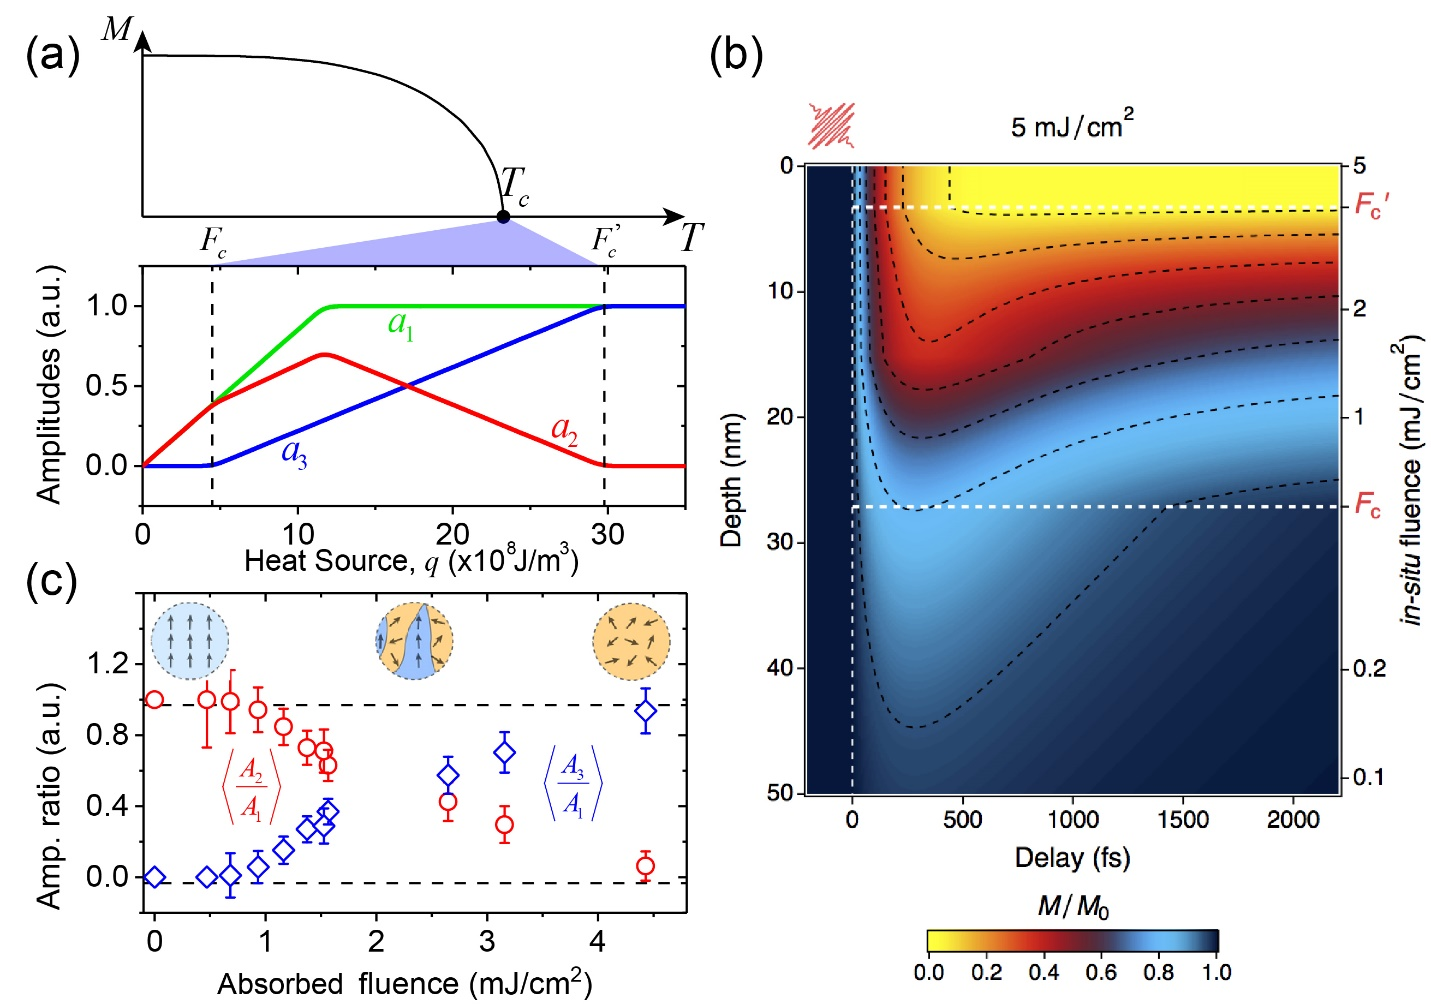
\includegraphics[width=150mm]{figs/PRLFig4}
\end{center}
\caption{(a) Top panel: Schematic magnetization of a ferromagnet as a function of temperature under thermal equilibrium with a single critical point ($T_c$). Bottom panel: Extracted amplitudes of the change of magnetization in a monolayer of Ni as a function of in-situ fluence and heat source. The correspondence of $T_c$ to the two critical fluences ($F_c$ and $F_c$') is highlighted. (b) The laser-induced magnetization variation in Ni as a function of time and depth. The black dashed lines represent the contours of equal magnetization. The white dashed lines separate different regions for the in-situ fluence relative to the two critical fluences $F_c$ and $F_c$'. (c) The relative contributions of the fast ($<A_3>$) recovery process directly extracted from the TR-TMOKE results in Fig. \ref{fig: PRLfig3}. Inset: Potential scenarios for the coexistence of ferromagnetic and paramagnetic phases in different fluence regions.}
\end{figure}

